In EDGE, registers are used to pass data between blocks.
To ensure that a younger block does not execute a register read on a register that must be written to by an older block, the register-file keeps track of registers which have to be written to.
If the younger block attempts to execute the read, its request is pushed back until the older block has executed its write and any instruction that depends on the read must wait until the read fires.
Whilst the serialisation of register reads and writes between blocks ensures correct execution of speculative blocks, it effectively reduces the potential for instruction level parallelism (ILP).
This is further exacerbated when fusing a large number of cores, as this increases the amount of blocks that may potentially have to wait on register reads and writes.

For example, the loop iterator in Listing~\ref{lst:basic} in Section~\ref{chp3:sec:fetch} is passed between iterations of the block through a register.
If multiple cores are composed, and all have an iteration of the loop, they may have to wait on previous writes to be able to execute their loads; serialising execution of the loop.
In situations where register dependencies are a bottleneck and cannot be optimised via a compiler, core composition cannot be considered an effective method of improving performance as the data dependencies serialise execution of blocks.

The problem of trying to reduce register and memory dependencies to improve instruction level parallelism is not new, and is an issue for more traditional superscalar processors~\cite{peraisVTAGE2014}.
For the loop in Listing~\ref{lst:basic}, the sole data dependency is found in the loop induction variable.
This variable is always incremented by 1, which means that given a block, the value can easily be predicted based on previous values of the variable.
In these cases value prediction can be used to attempt to ensure that these blocks can run in parallel even if there are dependencies.

\begin{figure}[t]
    \centering
    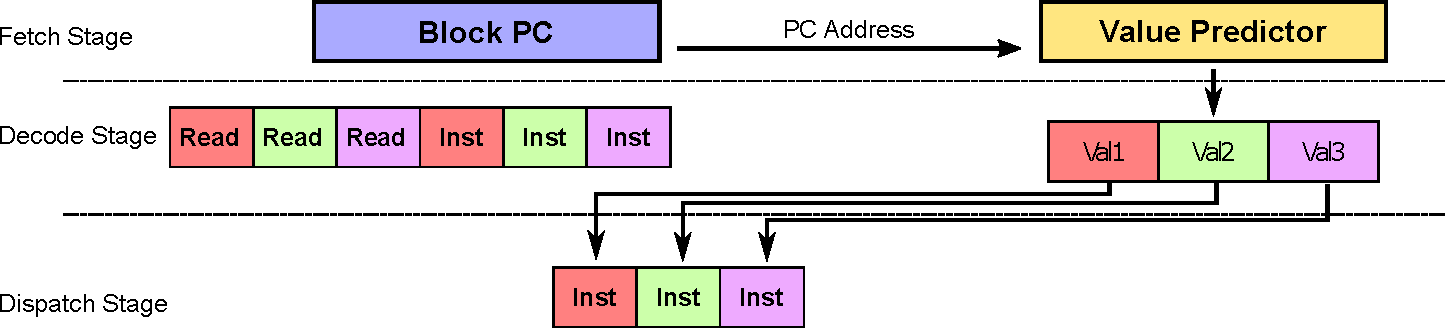
\includegraphics[width=1\textwidth]{chapter3/graphics/val_pred_overview.pdf}
    \caption{Overview of how a value predictor should work for EDGE. Prediction is made at the fetch stage, and predictions are used when register reads are dispatched.}
    \label{fig:bad_overview}
\vspace{1em}
\end{figure}

\subsection{Design features of a value predictor}

In this chapter, the only target for value predictions are register read instructions.
This is due to the fact that other instructions do not depend on previous blocks to fire, and load/store instructions can be fired independently unless dependencies are predicted.
Ideally, a value predictor for EDGE would function as seen in Figure~\ref{fig:bad_overview}; when a block is fetched, a single request is made to the value predictor to fetch all predictions for the read instructions of the block.
At dispatch time, the predicted values would be used and forwarded to instructions depending on a read, instead of issuing the read instructions.
This section covers different features that must be considered when implementing such a value predictor.


\paragraph*{Prediction Latency}
In a traditional superscalar processor, one of the main challenges value predictors face is being able to sustain the potential number of prediction requests in a short time frame~\cite{peraisBeBop2015}.
As value predictors are designed to improve ILP performance of out-of-order (OoO) superscalars, it is important to be able to issue a predicted value quickly.
If multiple prediction requests are made each cycle, this may require xpensive hardware such as a re-order buffer to hold all predictions~\cite{peraisBeBop2015}, which may dissuade designers from using value predictors.

To tackle the challenge of issuing predictions quickly, research has focussed on grouping instructions into prediction blocks~\cite{peraisBeBop2015}.
Instead of fetching a single prediction, each entry in the value predictor represents a set of predictions.
Entries are accessed by using the PC of the first instruction in a fetch block.
By grouping multiple predictions into a single entry, it drastically reduces the amount of requests to the value predictor, reducing the prediction latency for a large amount of instructions.
However, a block-based value predictor requires that the size of a block be determined at design time, which adds a new design task: choosing a small block size will increase the number of requests per cycle, whilst a large block size will decrease the number of entries and thus reduce overall accuracy.
As EDGE organises instructions as blocks, a block-based predictor would reduce the number of prediction requests per cycle, making it an attractive feature.


\paragraph*{Prediction generation} Another important feature when selecting a value predictor is how it generates a predicted value.
As of the writing of this thesis, there exist two main methods: direct value prediction~\cite{peraisVTAGE2014} and stride-based value prediction~\cite{peraisBeBop2015}.
The direct value predictor is the simpler design, as it only stores the last retired value for the specific instruction.
When a request is made, the direct value predictor will simply submit the last value.
Whilst this makes a value predictor small easy to design, such implementation is known to have poor accuracy when predicting values that are modified in quick succession.

On the other hand, stride-based value predictors use two components to make a prediction.
The first component is a Last-Value Table (LVT) which holds the last retired value for the instruction.
The second component is a stride, which represents the delta between the last two retired values for the instruction.
When a prediction is made, the value predictor fetches the value from the LVT, and adds the stride to make a prediction.
Such a design may increase the memory footprint as it has to store both a value and a stride for each data point; however it improves the overall accuracy and usefulness of value predictors.
It is also more accurate when executing loops as it can detect the stride at which the register values are modified.
As core composition is best used when executing loops, a stride-based predictor is recommended.

\paragraph*{Summary}

A perfect value predictor for EDGE must therefore be able to provide predictions in groups, as EDGE organises its instructions in blocks as this reduces the number of prediction requests per cycle.
Also, as value prediction is to be used in core compositions, a stride-based predictor is more adequate than a context based one.
Perais et al. propose such a predictor: a block based differential Value TAGE predictor~\cite{peraisBeBop2015}.
The next section covers briefly how this predictor works.

\subsection{Block based D-VTAGE predictor}

In this chapter, a block based differential value TAGE (D-VTAGE) predictor is implemented, based on the work of Perais et al.~\cite{peraisBeBop2015}.
Full details on how such a value predictor works can be found in Chapter~\ref{chp:Background} Section~\ref{chp:bck:vtage}.
To summarise, D-VTAGE is a stride based value predictor, which means that a prediction is composed of the last seen value for the instruction (found in a Last Value Table (LVT)), and a stride which represents the delta between the last two values for the instruction.
When a prediction is made, the last seen value and stride are added together to make the predicted value.

The predictor must also handle the fact that multiple blocks may be in flight, and thus the value found in the LVT may not be up to date.
In order to handle multiple in-flight predictions, D-VTAGE also contains a speculative window that has its own LVT that is speculatively updated when new predictions are made.
This allows the predictor to be able to handle situations where mutliple iterations of a loop are in flight.

Instead of issuing a single prediction per request, the block based D-VTAGE predictor issues multiple predictions for a single request.
This is an ideal mechanism when considering EDGE is the targetted platform.
In this case, when an EDGE block is fetched, a single request has to be made to the predictor to fetch all predictions for register reads.

Finally, as EDGE blocks are single entry, multiple exits, this simplifies the update mechanism for the Speculative Window.
In the original proposal of D-VTAGE by Perais et al.~\cite{peraisBeBop2015} they discuss the issue of how to handle updates in the Speculative Window after a flush.
This is due to the fact that in a traditional x86 environment, instructions being fetched after a flush may belong to a block of instructions that initiated the flush.
As this is not possible in EDGE, since whole blocks are flushed and fetched, there is no need for a complicated update policy.
Instead, a new prediction is always made when a block is fetched.


%\subsection{Perfect Value Predictor}

%The perfect value predictor is implemented using traces of the application being executed.
%When a new block is fetched, it querries the trace file and looks for the values of all the registers which will be read.
%When the block can execute a read, the simulator then feeds the register directly into the instruction operands, instead of querying the register file.

%The perfect value predictor has no hardware restriction as to fully capture the potential performance improvements.
%Thus, all the registers in a block can be predicted.
%More on how restricting the number of values which can be predicted per block is discussed in the analysis in Section~\ref{chp:chp3:sec:analysis}.
